% answers.tex —— 1999 年·上海卷·文史类 · 参考答案与详细解析片段
% 由 tools/generate_projects.py 依来源总账自 1999/1999_数学真题_上海文_试题.md + 1999/1999_数学真题_上海文_解析正文.md + 1999/1999_数学真题_上海文_答案要点.md 生成，勿手改（改源 MD 后重跑）


\begin{gktip}
本文以固定扫描件题面为计算对象，卷内答案只作为独立对照。Q13 与 Q19 的源题面/卷内答案冲突继续标为未决；题面与卷内答案均不得据推导擅改。Q8、Q20、Q21 的源图已目视复核并重绘为 TikZ；Q21 截面图标签 $P$ 的含义未由题干定义，保留待核。
\end{gktip}

\gkpart{一、填空题}

\begin{answer}
\gksolhead{1}{}

\textbf{题目}：

$\operatorname{tg}\left[\arccos\frac{\sqrt2}{2}-\frac\pi6\right]=$ \gkblank{}。

\Needspace{4\baselineskip}
\textbf{解析}

\Needspace{5\baselineskip}
由 $\arccos\frac{\sqrt2}{2}=\frac\pi4$，原式为
\nopagebreak[4]
\[
\tan\left(\frac\pi4-\frac\pi6\right)=\tan\frac\pi{12}=2-\sqrt3.
\]

\gkanswer{答案：$2-\sqrt3$}

\end{answer}
\begin{answer}
\gksolhead{2}{}

\textbf{题目}：

函数 $f(x)=\log_2 x+1\ (x\ge4)$ 的反函数 $f^{-1}(x)$ 的定义域是 \gkblank{}。

\Needspace{4\baselineskip}
\textbf{解析}

当 $x\ge4$ 时，$f(x)=\log_2x+1\ge3$，且函数递增，故反函数定义域（即原函数值域）为 $[3,+\infty)$。

\gkanswer{答案：$[3,+\infty)$（值域按数学定义不含 $+\infty$；扫描件右括号形似方括号）}

\end{answer}
\begin{answer}
\gksolhead{3}{}

\textbf{题目}：

在 $\left(x^3+\frac{2}{x^2}\right)^5$ 的展开式中，含 $x^5$ 项的系数为 \gkblank{}。

\Needspace{4\baselineskip}
\textbf{解析}

\Needspace{5\baselineskip}
二项展开通项为
\nopagebreak[4]
\[
\binom5k(x^3)^{5-k}\left(\frac2{x^2}\right)^k
=\binom5k2^k x^{15-5k}.
\]
令 $15-5k=5$，得 $k=2$，系数为 $\binom{5}{2}2^2=40$。

\gkanswer{答案：$40$}

\end{answer}
\begin{answer}
\gksolhead{4}{}

\textbf{题目}：

在 $\triangle ABC$ 中，若 $\angle B=30^\circ$，$AB=2\sqrt3$，$AC=2$，则 $\triangle ABC$ 的面积 $S$ 是 \gkblank{}。

\Needspace{4\baselineskip}
\textbf{解析}

\Needspace{5\baselineskip}
令 $BC=a$。由余弦定理
\nopagebreak[4]
\[
AC^2=AB^2+BC^2-2(AB)(BC)\cos B
\]
\Needspace{5\baselineskip}
得 $4=12+a^2-6a$，即 $(a-2)(a-4)=0$。两种正值均形成非退化三角形，故
\nopagebreak[4]
\[
S=\frac12(AB)(BC)\sin B=\frac{\sqrt3}{2}a\in\{\sqrt3,2\sqrt3\}.
\]

\gkanswer{答案：$\sqrt3$ 或 $2\sqrt3$}

\end{answer}
\begin{answer}
\gksolhead{5}{}

\textbf{题目}：

若平移坐标系，将曲线方程 $y^2+4x-4y-4=0$ 化为标准方程，则坐标原点应移到点 $O'(\underline{\qquad},\underline{\qquad})$。

\Needspace{4\baselineskip}
\textbf{解析}

\Needspace{5\baselineskip}
配方得
\nopagebreak[4]
\[
(y-2)^2=-4(x-2).
\]
新坐标原点应取在旧坐标 $(2,2)$，即 $O'(2,2)$。

\gkanswer{答案：$(2,2)$}

\end{answer}
\begin{answer}
\gksolhead{6}{}

\textbf{题目}：

函数 $y=2\sin x\cos x-2\sin^2x+1$ 的最小正周期 $T=$ \gkblank{}。

\Needspace{4\baselineskip}
\textbf{解析}

\Needspace{5\baselineskip}
利用 $2\sin x\cos x=\sin2x$、$1-2\sin^2x=\cos2x$，得
\nopagebreak[4]
\[
y=\sin2x+\cos2x=\sqrt2\sin\left(2x+\frac\pi4\right),
\]
其最小正周期为 $\pi$。

\gkanswer{答案：$\pi$}

\end{answer}
\begin{answer}
\gksolhead{7}{}

\textbf{题目}：

函数 $y=2\sin\left(2x+\frac\pi6\right)\ (x\in[-\pi,0])$ 的单调递减区间是 \gkblank{}。

\Needspace{4\baselineskip}
\textbf{解析}

\nopagebreak[4]
\[
y'=4\cos\left(2x+\frac\pi6\right).
\]
\Needspace{5\baselineskip}
在给定域 $x\in[-\pi,0]$ 内，导数非正对应
\nopagebreak[4]
\[
2x+\frac\pi6\in\left[-\frac{3\pi}{2},-\frac\pi2\right],
\]
所以函数在 $\left[-\frac{5\pi}{6},-\frac\pi3\right]$ 上递减。卷内所写为去掉两个端点的开区间；端点处导数为零但不影响区间上的严格递减。

\gkanswer{答案：$(-\frac{5\pi}{6},-\frac\pi3)$（卷内记开区间；在题给闭域上也严格递减）}

\end{answer}
\begin{answer}
\gksolhead{8}{}

\textbf{题目}：

某工程的工序流程图如下（工时单位：天）。
\nopagebreak[4]
\begin{center}% 1999 上海文科 Q8：按固定扫描页重绘；实线为工序，虚线为零工时虚活动。
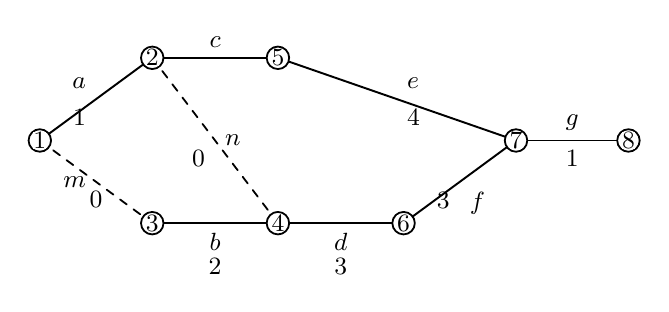
\begin{tikzpicture}[>=stealth, line join=round, line cap=round, scale=0.84,
  every node/.style={font=\small}]
  \tikzset{activity/.style={->, line width=0.7pt}, dummy/.style={->, dashed, line width=0.65pt}}
  \coordinate (n1) at (0,0);
  \coordinate (n2) at (1.7,1.25);
  \coordinate (n3) at (1.7,-1.25);
  \coordinate (n4) at (3.6,-1.25);
  \coordinate (n5) at (3.6,1.25);
  \coordinate (n6) at (5.5,-1.25);
  \coordinate (n7) at (7.2,0);
  \coordinate (n8) at (8.9,0);

  \draw[activity] (n1)--node[above left] {$a$} node[below left] {$1$} (n2);
  \draw[dummy] (n1)--node[left] {$m$} node[below] {$0$} (n3);
  \draw[activity] (n3)--node[below] {$b$} node[below=9pt] {$2$} (n4);
  \draw[dummy] (n2)--node[right] {$n$} node[below left] {$0$} (n4);
  \draw[activity] (n2)--node[above] {$c$} (n5);
  \draw[activity] (n4)--node[below] {$d$} node[below=9pt] {$3$} (n6);
  \draw[activity] (n5)--node[above right] {$e$} node[below right] {$4$} (n7);
  \draw[activity] (n6)--node[below right] {$f$} node[below left] {$3$} (n7);
  \draw[activity] (n7)--node[above] {$g$} node[below] {$1$} (n8);

  \foreach \name in {n1,n2,n3,n4,n5,n6,n7,n8} {
    \draw[fill=white, line width=0.65pt] (\name) circle (0.17);
  }
  \node[fill=white,inner sep=0pt] at (n1) {1};
  \node[fill=white,inner sep=0pt] at (n2) {2};
  \node[fill=white,inner sep=0pt] at (n3) {3};
  \node[fill=white,inner sep=0pt] at (n4) {4};
  \node[fill=white,inner sep=0pt] at (n5) {5};
  \node[fill=white,inner sep=0pt] at (n6) {6};
  \node[fill=white,inner sep=0pt] at (n7) {7};
  \node[fill=white,inner sep=0pt] at (n8) {8};
\end{tikzpicture}
\end{center}
\nopagebreak[4]
来源流程图的实线箭头为 $1\to2$（工序 $a$，工时 1）、$3\to4$（工序 $b$，工时 2）、$2\to5$（工序 $c$，图中未标工时）、$4\to6$（工序 $d$，工时 3）、$5\to7$（工序 $e$，工时 4）、$6\to7$（工序 $f$，工时 3）、$7\to8$（工序 $g$，工时 1）；虚线箭头为 $1\to3$（工序 $m$，工时 0）及 $2\to4$（工序 $n$，工时 0）。箭头方向、节点编号及工时按固定扫描记录，配图已与固定扫描页复核并纳入四版生成及本批次视觉校样。

现已知工程总时数为 10 天，则工序 $c$ 所需工时为 \gkblank{}。

\Needspace{4\baselineskip}
\textbf{解析}

\Needspace{5\baselineskip}
按源流程图列三条到终点的关键路径：
\nopagebreak[4]
\[
\begin{aligned}
1\to2\to5\to7\to8 &: c+6,\\
1\to2\to4\to6\to7\to8 &: 8,\\
1\to3\to4\to6\to7\to8 &: 9.
\end{aligned}
\]
总工期为三者最大值10天，故 $c+6=10$，得 $c=4$ 天。该推导依赖题面图中实线/虚线箭头与工时记录准确；这些标注已与固定扫描页交叉核看。

\gkanswer{答案：$4$ 天}

\end{answer}
\begin{answer}
\gksolhead{9}{}

\textbf{题目}：

$\dfrac{\log_3 2}{\log_{27}64}=$ \gkblank{}。

\Needspace{4\baselineskip}
\textbf{解析}

\nopagebreak[4]
\[
\log_{27}64=\frac{6\ln2}{3\ln3}=2\log_3 2,
\]
故所求比值为 $\frac12$。

\gkanswer{答案：$\frac12$}

\end{answer}
\begin{answer}
\gksolhead{10}{}

\textbf{题目}：

在等差数列 $\{a_n\}$ 中满足 $3a_4=7a_7$，且 $a_1>0$，$S_n$ 是数列 $\{a_n\}$ 前 $n$ 项的和。若 $S_n$ 取得最大值，则 $n=$ \gkblank{}。

\Needspace{4\baselineskip}
\textbf{解析}

\Needspace{5\baselineskip}
设公差为 $d$，则
\nopagebreak[4]
\[
3(a_1+3d)=7(a_1+6d)\implies d=-\frac{4a_1}{33}<0.
\]
\Needspace{5\baselineskip}
所以
\nopagebreak[4]
\[
a_n=a_1+(n-1)d=\frac{37-4n}{33}a_1.
\]
有 $a_9>0$ 而 $a_{10}<0$，故部分和在增加到第9项后开始下降，最大值于 $n=9$ 取得。

\gkanswer{答案：$9$}

\end{answer}
\begin{answer}
\gksolhead{11}{}

\textbf{题目}：

若以连续掷两次骰子分别得到的点数 $m,n$ 作为点 $P$ 的坐标，则点 $P$ 落在圆 $x^2+y^2=16$ 内的概率是 \gkblank{}。

\Needspace{4\baselineskip}
\textbf{解析}

两次掷骰子产生36个等可能有序点 $(m,n)$。满足 $m^2+n^2<16$ 的点为：$m=1$ 时 $n=1,2,3$；$m=2$ 时 $n=1,2,3$；$m=3$ 时 $n=1,2$，共8个。因此概率为 $8/36=2/9$。

\gkanswer{答案：$\frac29$}

\end{answer}
\begin{answer}
\gksolhead{12}{}

\textbf{题目}：

若四面体各棱的长是 1 或 2，且该四面体不是正四面体，则其体积的值是 \gkblank{}（只需写出一个可能的值）。

\Needspace{4\baselineskip}
\textbf{解析}

\Needspace{5\baselineskip}
取底面为边长1的正三角形，顶点到底面三顶点的棱均取2。底面外心到顶点距离为 $1/\sqrt3$，四面体高为
\nopagebreak[4]
\[
h=\sqrt{2^2-\frac13}=\sqrt{\frac{11}{3}}.
\]
\Needspace{5\baselineskip}
于是体积
\nopagebreak[4]
\[
V=\frac13\cdot\frac{\sqrt3}{4}\cdot\sqrt{\frac{11}{3}}=\frac{\sqrt{11}}{12}.
\]
所用六条棱均为1或2，且并非正四面体，符合题意。

\gkanswer{答案：$\frac{\sqrt{11}}{12}$（一个可实现的体积）}

\end{answer}
\gkpart{二、选择题}

\begin{answer}
\gksolhead{13}{}

\textbf{题目}：

直线 $y=-\frac{\sqrt3}{3}x$ 绕原点按逆时针方向旋转 $30^\circ$ 后所得直线与圆 $(x-2)^2+y^2=3$ 的位置关系是\mbox{（　　）}。

（A）直线过圆心；

（B）直线与圆相交，但不过圆心；

（C）直线与圆相切；

（D）直线与圆没有公共点。

\Needspace{4\baselineskip}
\textbf{解析}

原直线方向角可取 $-30^\circ$。逆时针旋转 $30^\circ$ 后成为 $y=0$。圆心为 $(2,0)$，故旋转后直线经过圆心，按题面选项应为 \textbf{A}。卷内答案表印 \textbf{C}（相切），与几何计算冲突，登记为来源答案冲突，暂不择一。

\gkanswer{答案：U/PENDING；冲突待核（卷内 C、按题面 A）}

\end{answer}
\begin{answer}
\gksolhead{14}{}

\textbf{题目}：

下列以 $t$ 为参数的参数方程所表示的曲线中，与方程 $xy=1$ 所表示的曲线完全一致的是\mbox{（　　）}。

（A）$\begin{cases}x=t^{1/2},\\y=t^{-1/2};\end{cases}$

（B）$\begin{cases}x=|t|,\\y=\dfrac1{|t|};\end{cases}$

（C）$\begin{cases}x=\cos t,\\y=\sec t;\end{cases}$

（D）$\begin{cases}x=\operatorname{tg}t,\\y=\operatorname{ctg}t.\end{cases}$

\Needspace{4\baselineskip}
\textbf{解析}

曲线 $xy=1$ 上 $x$ 可取任意非零实数。选项D令 $x=\operatorname{tg}t$、$y=\operatorname{ctg}t$，覆盖任意非零实数 $x$ 且 $xy=1$；A、B只给第一象限分支，C受 $|x|\le1$ 限制。因此选 \textbf{D}。

\gkanswer{答案：D}

\end{answer}
\begin{answer}
\gksolhead{15}{}

\textbf{题目}：

若 $a<b<0$，则下列结论中正确的是\mbox{（　　）}。

（A）不等式 $\frac1a>\frac1b$ 和 $\frac1{|a|}>\frac1{|b|}$ 均不能成立；

（B）不等式 $\frac1{a-b}>\frac1a$ 和 $\frac1{|a|}>\frac1{|b|}$ 均不能成立；

（C）不等式 $\frac1{a-b}>\frac1a$ 和 $\left(a+\frac1b\right)^2>\left(b+\frac1a\right)^2$ 均不能成立；

（D）不等式 $\frac1{|a|}>\frac1{|b|}$ 和 $\left(a+\frac1b\right)^2>\left(b+\frac1a\right)^2$ 均不能成立。

\Needspace{4\baselineskip}
\textbf{解析}

\Needspace{5\baselineskip}
由 $a<b<0$ 得 $a-b<0$ 且 $|a|>|b|$，所以
\nopagebreak[4]
\[
\frac1{a-b}<\frac1a,\qquad \frac1{|a|}<\frac1{|b|}.
\]
B中的两个严格大于式均不成立，故选 \textbf{B}。其余选项包含至少一个可成立的不等式。

\gkanswer{答案：B}

\end{answer}
\begin{answer}
\gksolhead{16}{}

\textbf{题目}：

设有直线 $m,n$ 和平面 $\alpha,\beta$，则在下列命题中，正确的是\mbox{（　　）}。

（A）若 $m\parallel n$，$m\subset\alpha$，$n\subset\beta$，则 $\alpha\parallel\beta$；

（B）若 $m\perp\alpha$，$m\perp n$，$n\subset\beta$，则 $\alpha\parallel\beta$；

（C）若 $m\parallel n$，$n\perp\beta$，$m\subset\alpha$，则 $\alpha\perp\beta$；

（A）若 $m\parallel n$，$m\perp\alpha$，$n\perp\beta$，则 $\alpha\perp\beta$。（扫描件此项标签照录为 A，与首项重复。）

\Needspace{4\baselineskip}
\textbf{解析}

第三个命题中 $m\parallel n$ 且 $n\perp\beta$，所以 $m\perp\beta$；又 $m\subset\alpha$，平面 $\alpha$ 含有一条垂直于 $\beta$ 的直线，因此 $\alpha\perp\beta$，选 \textbf{C}。题面第四项标签扫描确印为“A”，但其内容是两平面法线平行，不成立垂直关系；保留该标签异常。

\gkanswer{答案：C（正确命题内容；扫描件末项仍照录标签 A）}

\end{answer}
\gkpart{三、解答题}

\begin{answer}
\gksolhead{17}{}

\textbf{题目}（本题满分 10 分）：

设集合 $A=\{x\mid |x-a|<2\}$，$B=\left\{x\mid\frac{2x-1}{x+2}<1\right\}$。若 $A\subseteq B$，求实数 $a$ 的取值范围。

\Needspace{4\baselineskip}
\textbf{解析}

\nopagebreak[4]
\[
\frac{2x-1}{x+2}<1\iff\frac{x-3}{x+2}<0\iff -2<x<3.
\]
所以 $B=(-2,3)$，而 $A=(a-2,a+2)$。开区间包含要求 $a-2\ge-2$、$a+2\le3$，故 $0\le a\le1$。

\gkanswer{答案：$0\le a\le1$}

\end{answer}
\begin{answer}
\gksolhead{18}{}

\textbf{题目}（本题满分 12 分）：

\Needspace{5\baselineskip}
设正数数列 $\{a_n\}$ 为一等比数列，且 $a_2=4$，$a_4=16$，求
\nopagebreak[4]
\[
\lim_{n\to\infty}\frac{\lg a_{n+1}+\lg a_{n+2}+\cdots+\lg a_{2n}}{n^2}\mbox{。}
\]

\Needspace{4\baselineskip}
\textbf{解析}

\Needspace{5\baselineskip}
等比数列各项为正，故公比 $q>0$，且
\nopagebreak[4]
\[
q^2=\frac{a_4}{a_2}=4\implies q=2,\qquad a_1=\frac{a_2}{q}=2,
\]
\Needspace{5\baselineskip}
从而 $a_n=2^n$。于是
\nopagebreak[4]
\[
\frac{\lg a_{n+1}+\cdots+\lg a_{2n}}{n^2}
=\frac{\sum_{k=n+1}^{2n}k\,\lg2}{n^2}
=\frac{((n+1+2n)n/2)\lg2}{n^2}
=\left(\frac32+\frac1{2n}\right)\lg2.
\]
极限为 $\frac32\lg2$。

\gkanswer{答案：$\frac32\lg2$}

\end{answer}
\begin{answer}
\gksolhead{19}{}

\textbf{题目}（本题满分 14 分）：

设复数 $z$ 满足 $4z+2\bar z=3+\sqrt3+i$，$w=\sin\theta-i\cos\theta\ (\theta\in R)$，求 $z$ 的值和 $|z-w|$ 的取值范围。（原页参数域记号照录为 $R$。）

\Needspace{4\baselineskip}
\textbf{解析}

\Needspace{5\baselineskip}
令 $z=u+iv$。\textbf{按题面扫描的右端 $3+\sqrt3+i$}，有
\nopagebreak[4]
\[
6u+2iv=3+\sqrt3+i,
\]
\Needspace{5\baselineskip}
故 $z=\frac{3+\sqrt3}{6}+\frac12i$。设
\nopagebreak[4]
\[
r=|z|=\sqrt{\frac{7+2\sqrt3}{12}}<1.
\]
\Needspace{5\baselineskip}
因 $w=\sin\theta-i\cos\theta$ 遍历单位圆，固定点 $z$ 到单位圆上各点的距离范围是
\nopagebreak[4]
\[
|z-w|\in[1-r,1+r]
=\left[1-\sqrt{\frac{7+2\sqrt3}{12}},\,1+\sqrt{\frac{7+2\sqrt3}{12}}\right].
\]
\textbf{源冲突：}卷内解答把等式右端写成 $3\sqrt3+i$，得到 $z=\frac{\sqrt3}{2}+\frac12i$ 及范围 $[0,2]$。该解答对应另一右端，不能与本题面同时成立；维持未决，不用卷内解答替换题面。

\gkanswer{答案：未决（题面与卷内解答冲突；不得据此取单一答案）}

\end{answer}
\begin{answer}
\gksolhead{20}{}

\textbf{题目}（本题满分 16 分）：

本题共有 2 个小题，第 1 小题满分 4 分，第 2 小题满分 12 分。

如图，在四棱锥 $P-ABCD$ 中，底面 $ABCD$ 是一直角梯形，$\angle BAD=90^\circ$，$AD\parallel BC$，$AB=BC=a$，$AD=2a$，且 $PA\perp$ 底面 $ABCD$，$PD$ 与底面成 $30^\circ$ 角。

原卷图（印刷页 137）：
\nopagebreak[4]
\begin{center}% 1999 上海文科 Q20：依据固定扫描页的拓扑重绘；不表示长度/角度比例。
\begin{tikzpicture}[line join=round, line cap=round, scale=0.9]
  \tikzset{visible edge/.style={draw=black, line width=0.75pt}, hidden edge/.style={draw=black, dashed, line width=0.65pt}}
  \coordinate (P) at (0,3.05);
  \coordinate (A) at (0,0);
  \coordinate (B) at (-0.85,-1.65);
  \coordinate (C) at (1.45,-1.65);
  \coordinate (D) at (3.25,0.05);
  \coordinate (E) at (1.52,1.645);

  % Hidden base/back edges and the perpendicular projection to PD.
  \draw[hidden edge] (P)--(A);
  \draw[hidden edge] (A)--(B);
  \draw[hidden edge] (A)--(D);
  \draw[hidden edge] (A)--(E) (B)--(E);
  % Small right-angle marker at E, matching the original perpendicular mark.
  \draw[line width=0.55pt] (1.375,1.713)--(1.375,1.573)--(1.512,1.475);
  % Visible pyramid edges and front/right base edges.
  \draw[visible edge] (P)--(B);
  \draw[visible edge] (P)--(C);
  \draw[visible edge] (P)--(D);
  \draw[visible edge] (B)--(C);
  \draw[visible edge] (C)--(D);

  \node[above] at (P) {$P$};
  \node[below right=4pt] at (A) {$A$};
  \node[left=3pt] at (B) {$B$};
  \node[below] at (C) {$C$};
  \node[right] at (D) {$D$};
  \node[above right] at (E) {$E$};
  \node[below=12mm] at (1.15,-1.65) {示意图，不按比例};
\end{tikzpicture}
\end{center}
\nopagebreak[4]
图中按原页表达棱线遮挡与点 $E$ 的位置和扫描中可见的垂直标记，不按比例。

（1） 若 $AE\perp PD$，$E$ 为垂足，求证：$BE\perp PD$；

（2） 求异面直线 $AE$ 与 $CD$ 所成角的大小（用反三角函数表示）。

\Needspace{4\baselineskip}
\textbf{解析}

\Needspace{5\baselineskip}
取 $A=(0,0,0)$，令 $AB$、$AD$、$AP$ 分别为坐标轴方向，可设
\nopagebreak[4]
\[
B=(0,a,0),\ C=(a,a,0),\ D=(2a,0,0),\ P=\left(0,0,\frac{2a}{\sqrt3}\right),
\]
因为 $PA=AD\tan30^\circ=2a/\sqrt3$。

\gksubpart{(1)}

（1）$AB\perp AD$ 且 $AB\perp AP$，所以 $AB\perp$ 平面 $PAD$，从而 $AB\perp PD$。又 $AE\perp PD$，且 $AB$ 与 $AE$ 相交于 $A$，故 $PD\perp$ 平面 $ABE$，于是 $BE\perp PD$。

\gksubpart{(2)}

\Needspace{5\baselineskip}
（2）将 $A$ 投影到 $PD$ 得
\nopagebreak[4]
\[
E=\left(\frac a2,0,\frac{\sqrt3a}{2}\right),\quad
\overrightarrow{AE}=\left(\frac a2,0,\frac{\sqrt3a}{2}\right),\quad
\overrightarrow{CD}=(a,-a,0).
\]
\Needspace{5\baselineskip}
因此
\nopagebreak[4]
\[
\cos\theta=\frac{\overrightarrow{AE}\cdot\overrightarrow{CD}}
{|AE|\,|CD|}=\frac{1}{2\sqrt2}=\frac{\sqrt2}{4},
\]
异面直线所成角为 $\arccos\frac{\sqrt2}{4}$。

\gkanswer{答案（1）：$BE\perp PD$}

\gkanswer{答案（2）：$\arccos\frac{\sqrt2}{4}$}

\end{answer}
\begin{answer}
\gksolhead{21}{}

\textbf{题目}（本题满分 16 分）：

本题共有 3 个小题，第 1 小题满分 6 分，第 2 小题满分 4 分，第 3 小题满分 6 分。

平地上有一条水沟，沟沿是两条长 100 米的平行线段，沟宽 $AB$ 为 2 米，与沟沿垂直的平面与沟的交线是一段抛物线，抛物线顶点为 $O$，对称轴与地面垂直，沟深 1.5 米，沟中水深 1 米。

原卷图（印刷页 137）：
\nopagebreak[4]
\begin{center}% 1999 上海文科 Q21：保留水沟柱体与抛物线横截面的示意关系，不表示尺度。
\begin{tikzpicture}[line join=round, line cap=round, scale=0.82]
  \tikzset{visible edge/.style={draw=black, line width=0.75pt}, hidden edge/.style={draw=black, dashed, line width=0.65pt}}
  \coordinate (A)  at (0,0);
  \coordinate (B)  at (1.85,-0.55);
  \coordinate (O)  at (0.70,-1.75);
  \coordinate (A2) at (3.35,0.95);
  \coordinate (B2) at (5.20,0.35);
  \coordinate (O2) at (4.05,-1.10);
  \coordinate (M)  at (3.571,-0.088);

  % Near parabolic cross-section and prism length edges.
  \draw[visible edge] (A) .. controls (0.10,-0.90) and (0.33,-1.75) .. (O);
  \draw[visible edge] (O) .. controls (1.18,-1.75) and (1.68,-0.20) .. (B);
  \draw[visible edge] (A)--(A2);
  \draw[visible edge] (B)--(B2);
  \draw[visible edge] (O)--(O2);

  % The source shows the outer far profile, but its occluded inner segment is dashed.
  \draw[hidden edge] (A)--(B);
  \draw[visible edge] (A2) .. controls (3.425,0.615) and (3.495,0.245) .. (M);
  \draw[hidden edge] (M) .. controls (3.699,-0.647) and (3.843,-1.10) .. (O2);
  \draw[visible edge] (O2) .. controls (4.40,-1.10) and (4.90,-0.20) .. (B2);
  \draw[hidden edge] (A2)--(B2);

  \node[left] at (A) {$A$};
  \node[below=4pt] at (B) {$B$};
  \node[below] at (O) {$O$};
  \node[below=12mm] at (2.80,-1.75) {示意图，不按比例};
\end{tikzpicture}
\end{center}
\nopagebreak[4]
\nopagebreak[4]
\begin{center}% 1999 上海文科 Q21：抛物线横截面及原图所示等腰梯形改挖轮廓；标签 P 的含义未由题干定义；非比例示意。
\begin{tikzpicture}[line join=round, line cap=round, scale=1.05]
  \tikzset{source curve/.style={draw=black,line width=0.75pt}, overlay/.style={draw=black,dashed,line width=0.65pt}}
  \coordinate (A) at (-1.75,0);
  \coordinate (B) at (1.75,0);
  \coordinate (O) at (0,-1.85);
  \coordinate (L) at (-0.52,-1.48);
  \coordinate (R) at (0.52,-1.48);
  \draw[source curve] (A) .. controls (-1.10,-1.28) and (-0.48,-1.85) .. (O)
                          .. controls (0.48,-1.85) and (1.10,-1.28) .. (B);
  \draw[overlay] (A)--(B);
  \draw[overlay] (A)--(L)--(R)--(B);
  \node[above left] at (A) {$A$};
  \node[above right] at (B) {$B$};
  \node[below] at (O) {$O$};
  \node[right=2pt] at (0.88,-1.08) {$P$};
  \node[below=12pt] at (0,-2.06) {示意图，不按比例};
\end{tikzpicture}
\end{center}
\nopagebreak[4]
横截面还照录源图标签 $P$；其几何含义未在题干定义。图形表达固定扫描中的柱体、抛物线截面和梯形轮廓，不按比例。

（1） 求水面宽；

（2） 如图所示形状的几何体积为柱体。已知柱体的体积为底面面积乘以高。问沟中的水有多少立方米？（疑似源文排印问题，暂照录。）

（3） 若要把这条水沟改挖（不准填土）成截面为等腰梯形的沟，使沟的底面与地面平行，则改挖后的沟底宽为多少米时，所挖的土最少？

\Needspace{4\baselineskip}
\textbf{解析}

以抛物线顶点 $O$ 为原点、对称轴为 $y$ 轴。沟沿点的坐标可取 $(1,3/2)$，故横截面为 $y=\frac32x^2$。

\gksubpart{(1)}

（1）水深为1米，水面对应 $y=1$，交点 $x=\pm\sqrt{2/3}$，水面宽为 $2\sqrt6/3$ 米。

\gksubpart{(2)}

\Needspace{5\baselineskip}
（2）按源题柱体描述，沟沿长度100米且横截面不变。水的截面积为
\nopagebreak[4]
\[
A=\int_{-\sqrt{2/3}}^{\sqrt{2/3}}\left(1-\frac32x^2\right)dx
=\frac{4\sqrt6}{9}.
\]
水量为 $100A=\frac{400\sqrt6}{9}$ 立方米。题面“如图所示形状的几何体积为柱体”疑似有漏字；此计算以等截面柱体为前提。

\gksubpart{(3)}

（3）改挖的等腰梯形截面须包含原抛物线截面。其沟底不高于 $O$，而若低于 $O$，仍可上移到 $O$ 并减少面积，故最优底面经过 $O$，梯形高为 $3/2$。在半高 $y=3/4$ 处，原沟宽为 $\sqrt2$；任何包含原沟的梯形其中位线宽至少 $\sqrt2$。梯形面积等于高乘中位线长，故面积下界为 $\frac{3\sqrt2}{2}$。

\Needspace{5\baselineskip}
当等腰梯形两腰取抛物线在 $\left(\pm\frac1{\sqrt2},\frac34\right)$ 处的切线时达到该下界。右切线为
\nopagebreak[4]
\[
y=\frac3{\sqrt2}x-\frac34.
\]
与底面 $y=0$ 的交点横坐标为 $\frac{\sqrt2}{4}$，故沟底全宽为 $\frac{\sqrt2}{2}$ 米。

\gkanswer{答案（1）：$\frac{2\sqrt6}{3}$ 米}

\gkanswer{答案（2）：$\frac{400\sqrt6}{9}$ 立方米（按等截面柱体解释）}

\gkanswer{答案（3）：$\frac{\sqrt2}{2}$ 米}

\end{answer}
\begin{answer}
\gksolhead{22}{}

\textbf{题目}（本题满分 18 分）：

本题共有 3 个小题，第 1 小题满分 6 分，第 2 小题满分 6 分，第 3 小题满分 6 分。

\Needspace{5\baselineskip}
设椭圆 $l$ 的方程为
\nopagebreak[4]
\[
\frac{(x+c)^2}{b^2}+\frac{(y+c)^2}{a^2}=1\mbox{，}
\]
其中 $a>b>0$，$c$ 为椭圆的半焦距。

（1） 将椭圆 $l$ 绕它的上焦点按逆时针方向旋转 $\frac\pi2$，求所得椭圆 $L$ 的中心的坐标、长轴长、短轴长及其方程；

（2） 若椭圆 $L$ 与曲线 $y=\frac1x$ 在第一象限内只有一个公共点 $P$，试用 $a$ 表示点 $P$ 的坐标；

（3） 设 $A\text{、}B$ 是椭圆 $L$ 的两个焦点，当 $a$ 变化时，求 $\triangle ABP$ 的面积函数 $S(a)$ 的值域。

\Needspace{4\baselineskip}
\textbf{解析}

\gksubpart{(1)}

\Needspace{5\baselineskip}
（1）椭圆 $l$ 的中心为 $(-c,-c)$，上焦点为 $(-c,0)$。中心相对该焦点的向量为 $(0,-c)$，逆时针旋转 $\pi/2$ 后为 $(c,0)$，所以新中心为原点；长短轴互换方向但长度不变，故
\nopagebreak[4]
\[
L:\quad\frac{x^2}{a^2}+\frac{y^2}{b^2}=1,
\]
长轴长为 $2a$、短轴长为 $2b$。

\gksubpart{(2)}

\Needspace{5\baselineskip}
（2）代入 $y=1/x$：
\nopagebreak[4]
\[
\frac{x^2}{a^2}+\frac{1}{b^2x^2}=1.
\]
\Needspace{5\baselineskip}
令 $t=x^2>0$，得 $t^2-a^2t+a^2/b^2=0$。第一象限只有一个交点，等价于该二次方程有一个正重根，因此判别式为0，得 $ab=2$。重根 $t=a^2/2$，所以
\nopagebreak[4]
\[
P=\left(\frac{a}{\sqrt2},\frac{\sqrt2}{a}\right).
\]
结合 $a>b=2/a$，参数域为 $a>\sqrt2$。

\gksubpart{(3)}

\Needspace{5\baselineskip}
（3）椭圆焦距半长为 $\sqrt{a^2-b^2}=\sqrt{a^2-4/a^2}$，三角形底边长为其两倍，高为 $\sqrt2/a$，故
\nopagebreak[4]
\[
S(a)=\frac12\cdot2\sqrt{a^2-\frac4{a^2}}\cdot\frac{\sqrt2}{a}
=\sqrt{2-\frac8{a^4}},\qquad a>\sqrt2.
\]
该函数从0单调增加并趋近 $\sqrt2$，两端均不能取得，故值域为 $(0,\sqrt2)$。

\gkanswer{答案（1）：中心 $(0,0)$，长轴 $2a$，短轴 $2b$，$\frac{x^2}{a^2}+\frac{y^2}{b^2}=1$}

\gkanswer{答案（2）：$P=\left(\frac a{\sqrt2},\frac{\sqrt2}{a}\right)$，$ab=2$，$a>\sqrt2$}

\gkanswer{答案（3）：$S(a)$ 的值域为 $(0,\sqrt2)$}

\end{answer}